% =====================================================================
% 슈퍼마켓 옴니채널 수요 예측 시스템 — 요약 보고서
% Compiled with: xelatex grocery_summary.tex
% =====================================================================
\documentclass[11pt, a4paper]{article}

% --- Fonts & Language ---
\usepackage{fontspec}
\usepackage{xetexko}

% --- Page geometry ---
\usepackage[margin=2.3cm, top=2.8cm, bottom=2.8cm]{geometry}

% --- Packages ---
\usepackage{graphicx}
\usepackage{booktabs}
\usepackage{tabularx}
\usepackage{xcolor}
\usepackage{hyperref}
\usepackage{titlesec}
\usepackage{fancyhdr}
\usepackage{float}
\usepackage{enumitem}
\usepackage{colortbl}
\usepackage{tikz}
\usepackage{setspace}
\usepackage{ragged2e}

% --- Font ---
\setmainfont{Apple SD Gothic Neo}

% --- Colors ---
\definecolor{darkblue}{HTML}{0F172A}
\definecolor{lightblue}{HTML}{D4E6F1}
\definecolor{accent}{HTML}{60A5FA}
\definecolor{red}{HTML}{DC2626}
\definecolor{gray}{HTML}{64748B}
\definecolor{kpibox}{HTML}{EBF5FB}
\definecolor{warnbox}{HTML}{FEF3C7}
\definecolor{greenbox}{HTML}{D1FAE5}
\definecolor{lightgray}{HTML}{F1F5F9}
\definecolor{bordergray}{HTML}{CBD5E1}
\definecolor{darkaccent}{HTML}{1E40AF}

% --- Hyperref ---
\hypersetup{
  colorlinks=true,
  linkcolor=darkaccent,
  urlcolor=accent,
  citecolor=darkblue,
  pdfborder={0 0 0}
}

% --- Section formatting ---
\titleformat{\section}
  {\Large\bfseries\color{darkblue}}
  {\thesection}{1em}{}
  [\vspace{-0.5em}\textcolor{accent}{\rule{\textwidth}{1.5pt}}]

\titleformat{\subsection}
  {\large\bfseries\color{darkblue}}
  {\thesubsection}{0.8em}{}

% --- Header / Footer ---
\pagestyle{fancy}
\fancyhf{}
\renewcommand{\headrulewidth}{0pt}
\fancyfoot[C]{\footnotesize\textcolor{gray}{한양대학교 경영대학 임보람 교수 연구실 \textperiodcentered{} 빅데이터 마케팅 연구그룹}}
\fancyfoot[R]{\footnotesize\textcolor{gray}{\thepage}}
\fancypagestyle{plain}{
  \fancyhf{}
  \renewcommand{\headrulewidth}{0pt}
  \fancyfoot[C]{\footnotesize\textcolor{gray}{한양대학교 경영대학 임보람 교수 연구실 \textperiodcentered{} 빅데이터 마케팅 연구그룹}}
  \fancyfoot[R]{\footnotesize\textcolor{gray}{\thepage}}
}

% --- Custom commands ---
\newcommand{\metriccard}[3]{%
  \begin{tikzpicture}
    \node[
      fill=kpibox,
      rounded corners=6pt,
      minimum width=4.8cm,
      minimum height=2.4cm,
      inner sep=8pt,
      align=center
    ] {
      {\small\textcolor{gray}{#1}}\\[3pt]
      {\LARGE\bfseries\textcolor{darkblue}{#2}}\\[2pt]
      {\footnotesize\textcolor{accent}{#3}}
    };
  \end{tikzpicture}%
}

\newcommand{\insightbox}[1]{%
  \vspace{0.5em}
  \noindent
  \fcolorbox{accent}{kpibox}{%
    \parbox{\dimexpr\textwidth-2\fboxsep-2\fboxrule}{%
      \vspace{0.4em}
      \textcolor{darkblue}{\textbf{핵심 인사이트}} \quad #1
      \vspace{0.4em}
    }%
  }%
  \vspace{0.5em}
}

\begin{document}

% =====================================================================
% COVER PAGE
% =====================================================================
\thispagestyle{empty}
\begin{tikzpicture}[remember picture, overlay]
  \fill[darkblue] (current page.north west) rectangle (current page.south east);
  \fill[accent] ([yshift=-9cm]current page.north west) rectangle ([yshift=-9.15cm]current page.north east);
  \fill[accent, opacity=0.3] ([yshift=3cm]current page.south west) rectangle ([yshift=3.08cm]current page.south east);
\end{tikzpicture}

\vspace*{4.5cm}

\begin{center}
  {\fontsize{30}{38}\selectfont\bfseries\textcolor{white}{슈퍼마켓 옴니채널}}\\[0.4cm]
  {\fontsize{30}{38}\selectfont\bfseries\textcolor{white}{수요 예측 시스템}}\\[0.8cm]
  {\fontsize{18}{26}\selectfont\bfseries\textcolor{accent}{온 \textperiodcentered{} 오프라인 채널별 카테고리 수요 예측}}\\[1.5cm]
  \textcolor{accent}{\rule{8cm}{0.8pt}}\\[1.5cm]
  {\fontsize{13}{18}\selectfont\textcolor{lightblue}{국내 대형 슈퍼마켓 체인 284개 매장 실증 분석}}\\[0.3cm]
  {\fontsize{13}{18}\selectfont\textcolor{lightblue}{온라인 예측 정확도 98.3\% 달성}}\\[2.5cm]
  {\fontsize{12}{16}\selectfont\textcolor{white}{한양대학교 경영대학}}\\[0.3cm]
  {\fontsize{13}{18}\selectfont\bfseries\textcolor{accent}{임보람 교수 연구실}}\\[0.3cm]
  {\fontsize{11}{15}\selectfont\textcolor{lightblue}{빅데이터 마케팅 연구그룹}}\\[2cm]
  {\footnotesize\textcolor{gray}{Summary Report \textperiodcentered{} JRCS Accepted}}
\end{center}

\newpage

% =====================================================================
% PAGE 2: EXECUTIVE SUMMARY
% =====================================================================
\section*{Executive Summary}

\vspace{0.5em}

온라인 채널 예측 정확도 \textbf{98.3\%} --- 국내 대형 슈퍼마켓 체인 \textbf{284개 매장}의 온 \textperiodcentered{} 오프라인 채널별 카테고리 수요를 AI 모델로 예측한다. 오프라인 채널 역시 87.3\%의 높은 정확도를 달성했다.

\vspace{1em}

\begin{center}
\metriccard{온라인 예측 정확도}{98.3\%}{채널별 수요 예측}
\hfill
\metriccard{오프라인 정확도}{87.3\%}{매장 수요 예측}
\hfill
\metriccard{분석 규모}{284 매장}{옴니채널 통합 분석}
\end{center}

\vspace{1em}

\insightbox{슈퍼마켓의 온라인과 오프라인 채널은 수요 동인이 근본적으로 다르다. 온라인은 편의성과 정기 구매 패턴이, 오프라인은 상권 특성과 경쟁 환경이 핵심 동인이다. 채널별 맞춤 예측이 통합 모델 대비 일관되게 우수하다.}

\vspace{0.5em}

\noindent\textcolor{gray}{\small 본 연구는 \textit{Journal of Retailing and Consumer Services} (JRCS)에 게재 승인되었습니다.}

\newpage

% =====================================================================
% PAGE 3: 채널별 예측 성능
% =====================================================================
\section*{채널별 예측 정확도}

\vspace{0.5em}

온라인 채널은 98.3\%, 오프라인 채널은 87.3\%의 예측 정확도를 달성했다. 이는 채널별 수요 특성을 반영한 맞춤형 모델링의 결과이다.

\vspace{1em}

\begin{figure}[H]
  \centering
  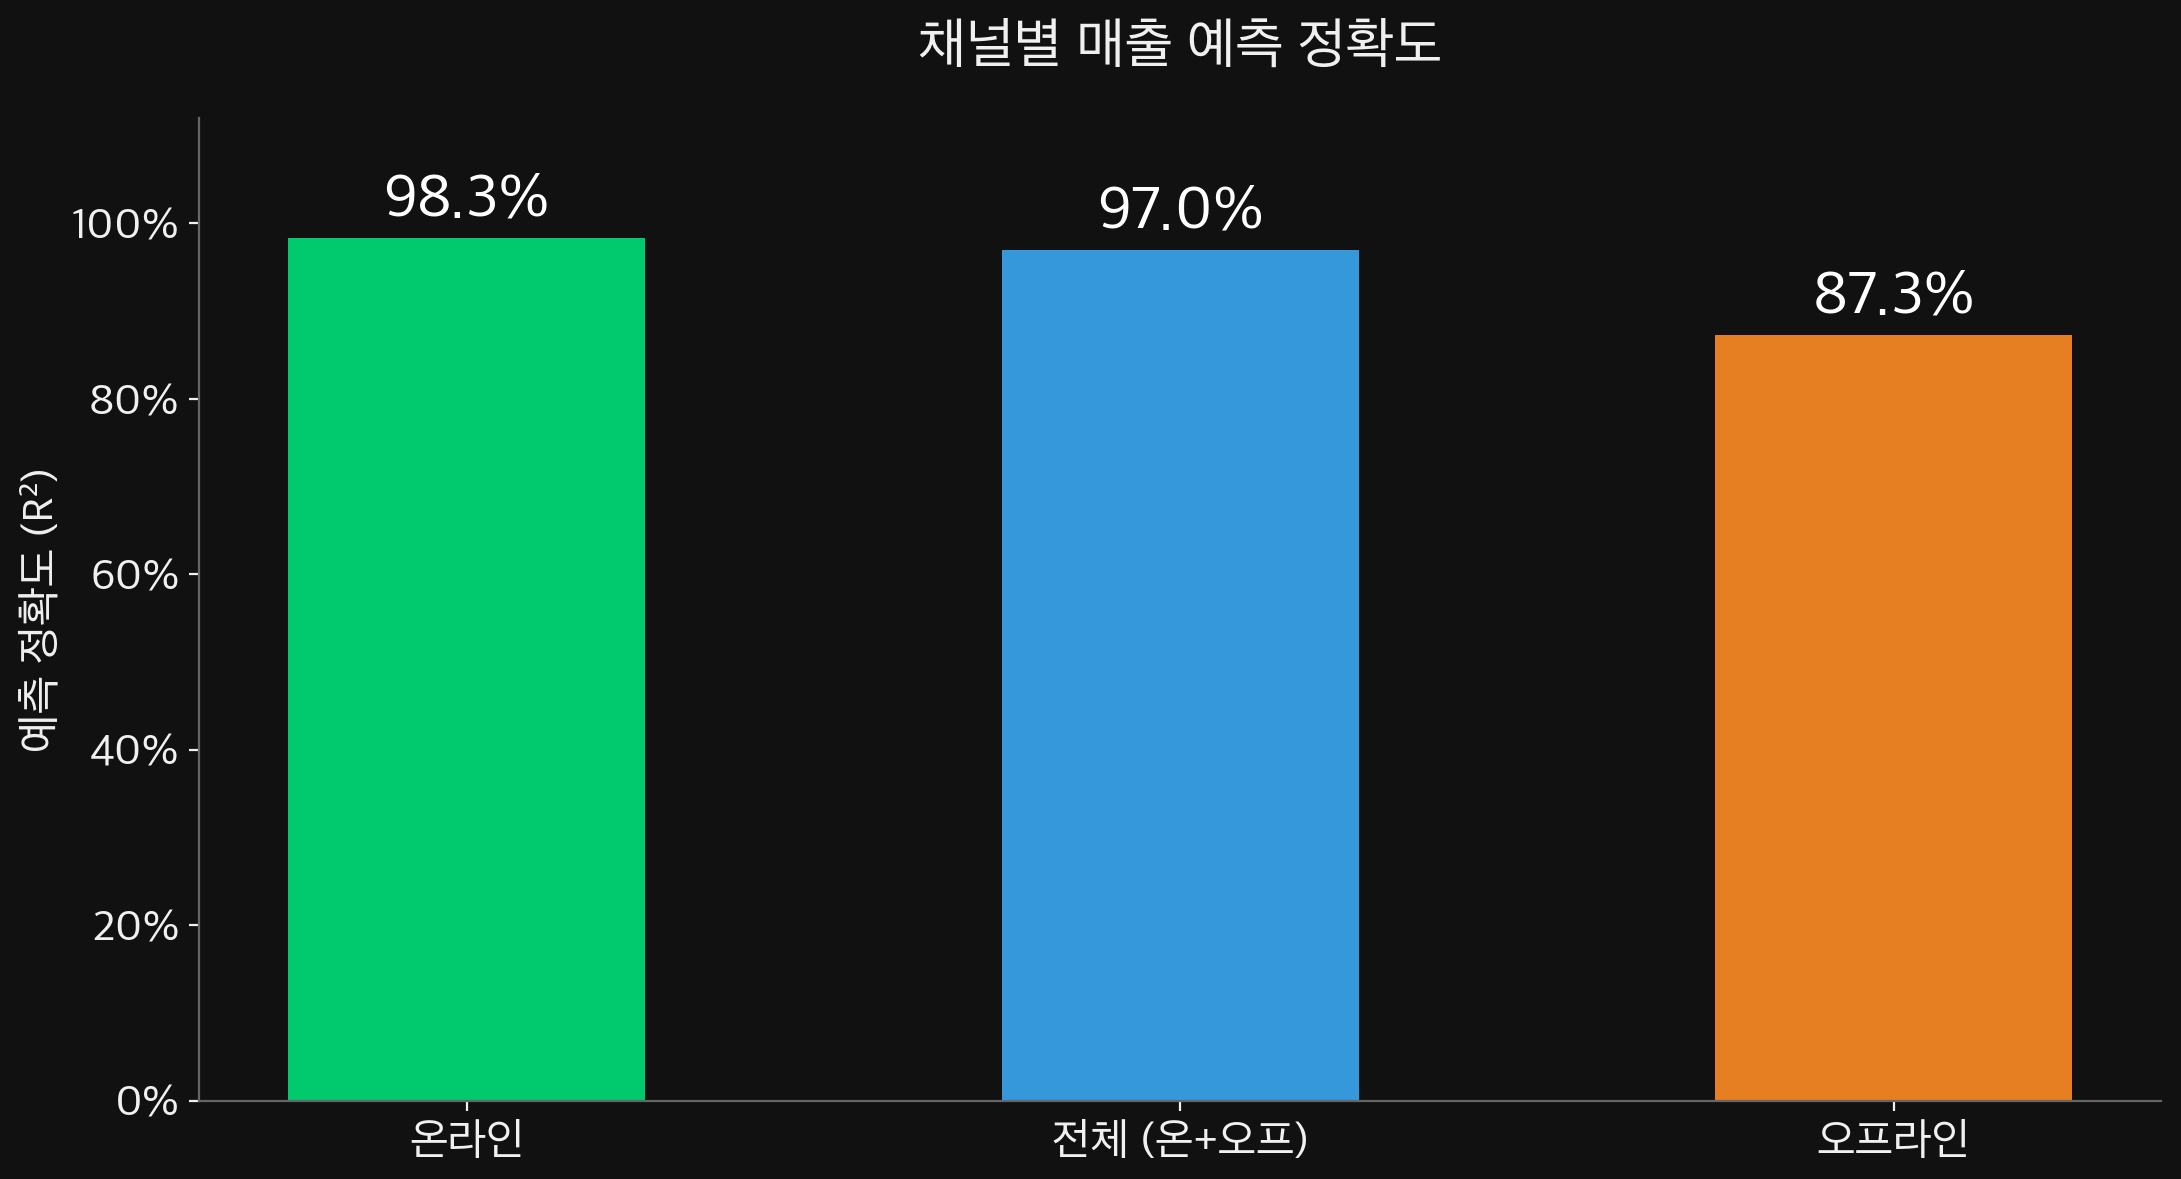
\includegraphics[width=0.92\textwidth]{v2_channel_accuracy.png}
  \caption{온 \textperiodcentered{} 오프라인 채널별 예측 정확도}
\end{figure}

\vspace{0.5em}

\insightbox{온라인 채널의 높은 예측 정확도(98.3\%)는 온라인 구매 행동의 패턴이 더 규칙적임을 보여준다. 이는 재고 관리 및 물류 최적화에 직접 활용 가능하다.}

\newpage

% =====================================================================
% PAGE 4: 카테고리 인사이트
% =====================================================================
\section*{카테고리별 수요 인사이트}

\vspace{0.5em}

상품 카테고리에 따라 수요 동인과 예측 패턴이 크게 다르다. 카테고리별 맞춤 전략이 전체 매출 최적화의 핵심이다.

\vspace{1em}

\begin{figure}[H]
  \centering
  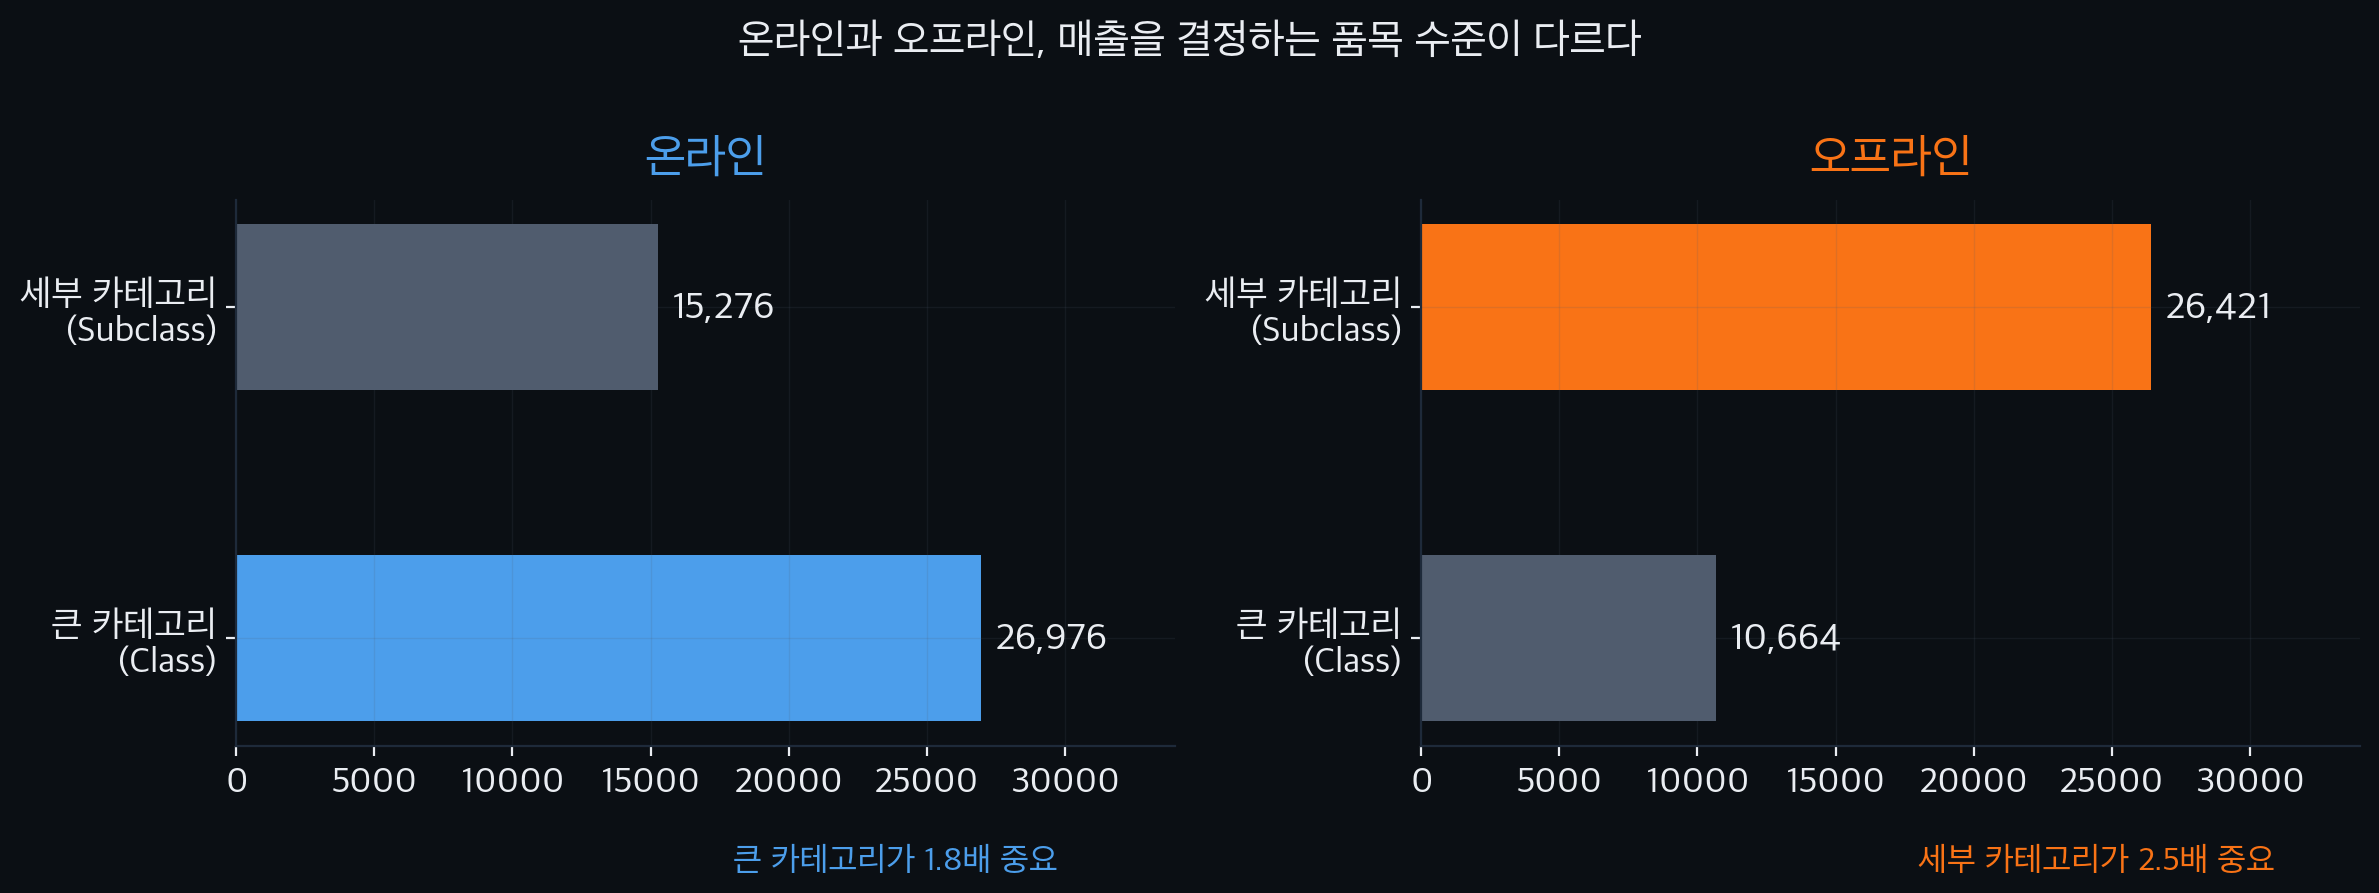
\includegraphics[width=0.92\textwidth]{web_category_insight.png}
  \caption{카테고리별 수요 예측 인사이트}
\end{figure}

\vspace{1em}

\begin{figure}[H]
  \centering
  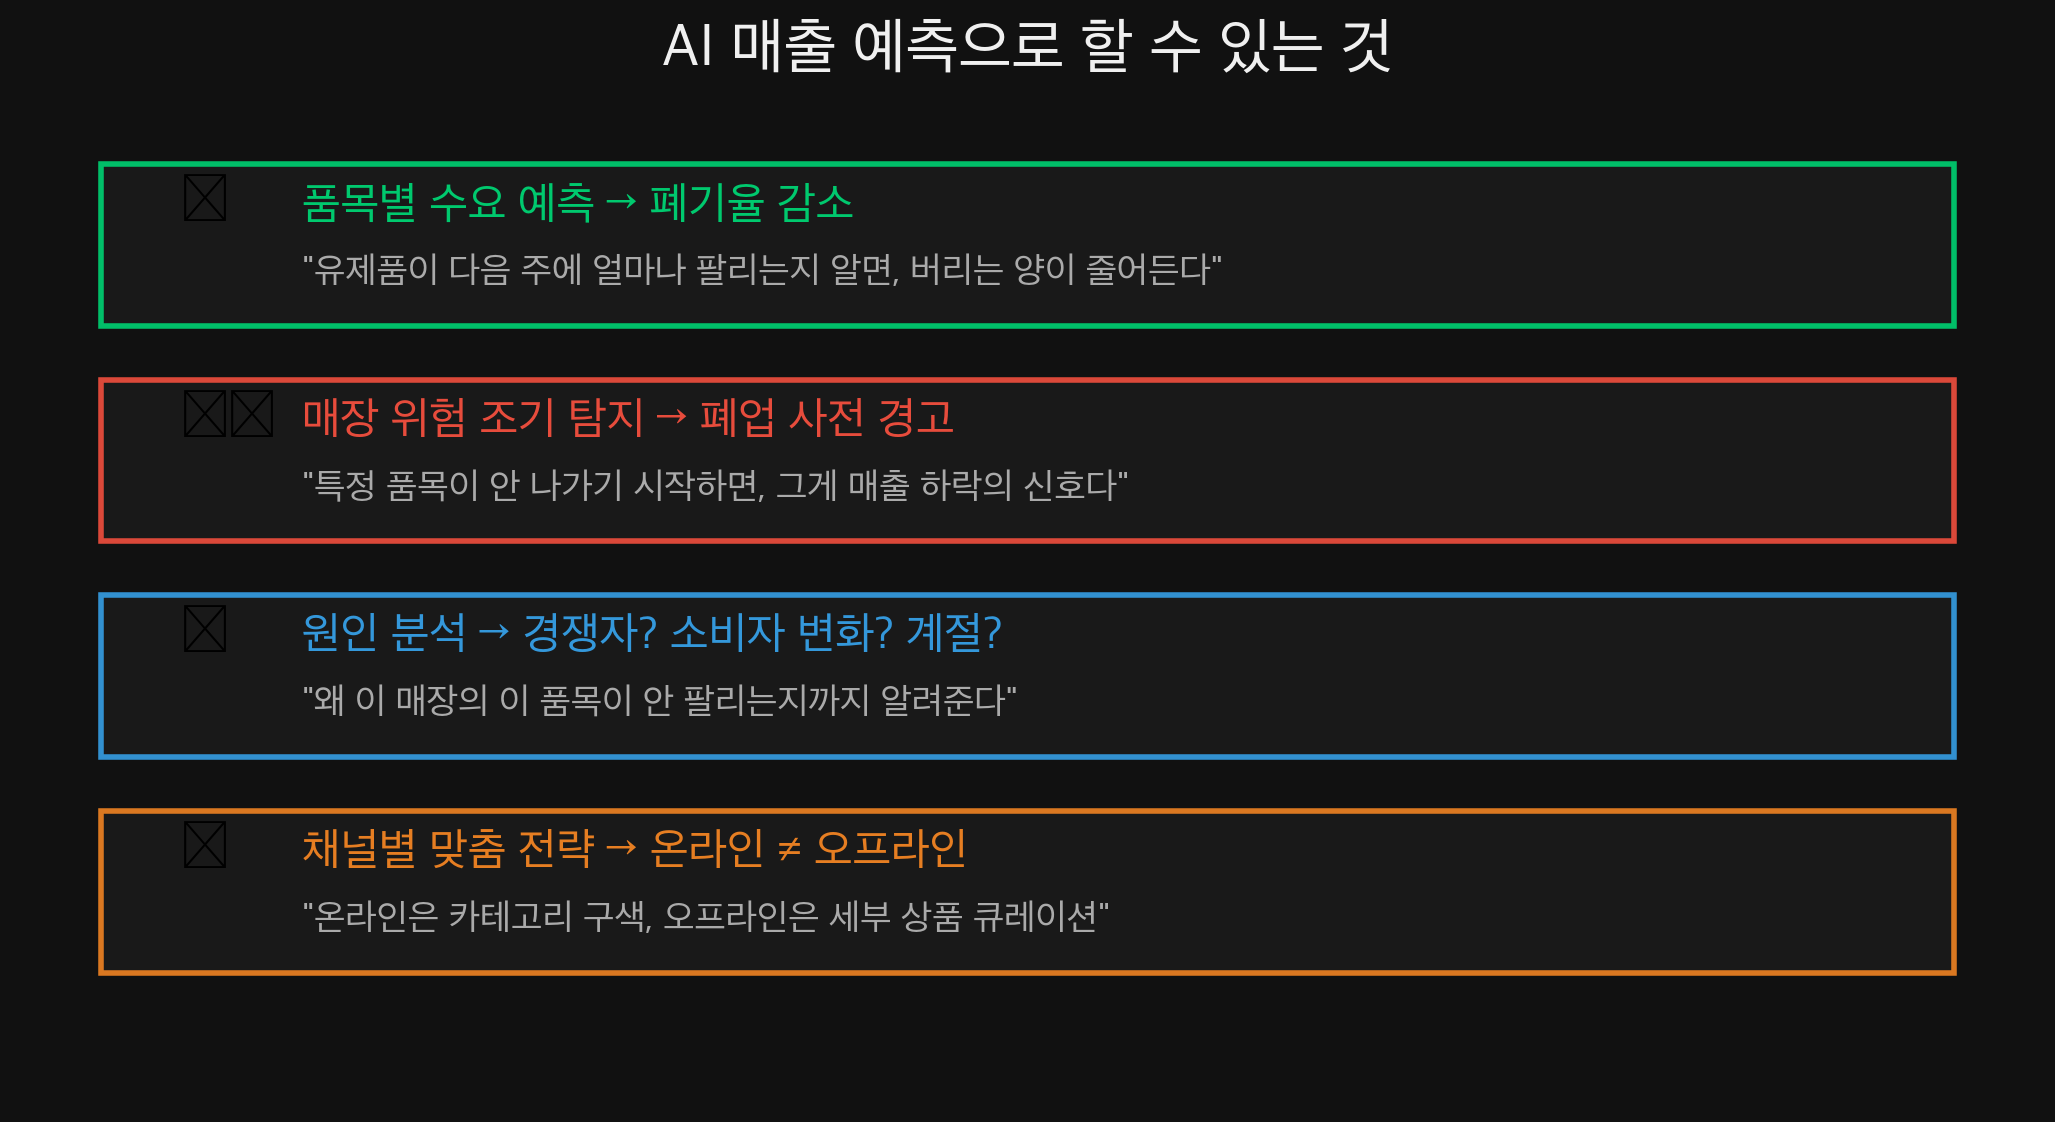
\includegraphics[width=0.92\textwidth]{v2_applications.png}
  \caption{수요 예측 시스템의 실무 적용 방안}
\end{figure}

\newpage

% =====================================================================
% PAGE 5: 전략적 시사점 + 문의
% =====================================================================
\section*{전략적 시사점}

\vspace{0.5em}

\noindent
\fcolorbox{bordergray}{lightgray}{%
  \parbox{\dimexpr\textwidth-2\fboxsep-2\fboxrule}{%
    \vspace{0.8em}
    {\large\bfseries\textcolor{darkblue}{1. 온라인 채널 재고 자동 관리}}\\[6pt]
    {\normalsize 98.3\% 정확도의 수요 예측 모델을 활용하면, 온라인 채널의 재고 수준을 자동으로 최적화할 수 있다. 과잉 재고와 품절을 동시에 줄여 비용 절감과 고객 만족을 달성한다.}
    \vspace{0.6em}
  }%
}

\vspace{0.8em}

\noindent
\fcolorbox{bordergray}{lightgray}{%
  \parbox{\dimexpr\textwidth-2\fboxsep-2\fboxrule}{%
    \vspace{0.8em}
    {\large\bfseries\textcolor{darkblue}{2. 카테고리별 프로모션 최적화}}\\[6pt]
    {\normalsize 카테고리마다 수요 동인이 다르므로, 카테고리별 맞춤 프로모션 전략이 전체 매출 극대화의 핵심이다. 수요 예측 모델로 프로모션 효과를 사전에 시뮬레이션할 수 있다.}
    \vspace{0.6em}
  }%
}

\vspace{0.8em}

\noindent
\fcolorbox{bordergray}{lightgray}{%
  \parbox{\dimexpr\textwidth-2\fboxsep-2\fboxrule}{%
    \vspace{0.8em}
    {\large\bfseries\textcolor{darkblue}{3. 옴니채널 통합 운영 전략}}\\[6pt]
    {\normalsize 온라인과 오프라인 채널의 수요 동인이 다르다는 실증 결과는, 채널별 차별화된 운영 전략의 필요성을 보여준다. 통합 예측 시스템으로 채널 간 시너지를 극대화할 수 있다.}
    \vspace{0.6em}
  }%
}

\vspace{3em}

\begin{center}
\fcolorbox{darkaccent}{lightblue}{%
  \parbox{0.85\textwidth}{%
    \vspace{1em}
    \begin{center}
    {\Large\bfseries\textcolor{darkblue}{전체 보고서 및 상세 분석은}}\\[8pt]
    {\Large\bfseries\textcolor{darkblue}{연구실로 문의해주세요}}\\[12pt]
    {\normalsize\textcolor{gray}{한양대학교 경영대학 임보람 교수 연구실}}\\[4pt]
    {\normalsize\textcolor{gray}{빅데이터 마케팅 연구그룹}}
    \end{center}
    \vspace{1em}
  }%
}
\end{center}

\end{document}
